\documentclass{bioinfo}
\copyrightyear{2008}
\pubyear{2008}
\usepackage{url}

\newif\ifnonbi
\nonbifalse
\newif\ifbi
\bitrue

\bibliographystyle{natbib}

\begin{document}
\firstpage{1}

\begin{application}

\title[Infernal 1.0]{Infernal 1.0: inference of RNA alignments}
\author[E. Nawrocki, D. Kolbe and S. Eddy]{Eric P. Nawrocki,\,$^1$ Diana L. Kolbe\,$^1$ and Sean R. Eddy\,$^1$\footnote{to whom correspondence should be addressed}}
\address{$^{1}$HHMI Janelia Farm Research Campus, Ashburn VA 20147, USA\\}

\history{Received on XXXXX; revised on XXXXX; accepted on XXXXX}

\editor{Associate Editor: XXXXXXX}

\maketitle

\begin{abstract}
\section{Summary:}
%\textsc{infernal} is a software package for building
\textsc{infernal} builds 
consensus RNA secondary structure profiles called covariance models
(CMs), and uses them to search nucleic acid sequence databases for
%(CMs), and using them to search nucleic acid sequence databases for
homologous RNAs, or to create new sequence and structure-based
multiple sequence alignments.

\section{Availability:}
Source code and documentation downloadable from
\href{http://infernal.janelia.org}. Freely licensed under the GNU
General Public License version 3 (GPLv3).

%\section{Contact:} \href{\{nawrockie,kolbed,eddys\}@janelia.hhmi.org}
\section{Contact:} \url{{nawrockie,kolbed,eddys}@janelia.hhmi.org}
\end{abstract}

\section{Introduction}

\software{infernal} is a software package that allows you to make
consensus RNA secondary structure profiles, and use them to search
nucleic acid sequence databases for homologous RNAs, or to create new
structure-based multiple sequence alignments.

To make a profile, you need to have a multiple sequence alignment of
an RNA sequence family, and the alignment must be annotated with a
consensus RNA secondary structure. The program \prog{cmbuild} takes an
annotated multiple alignment as input, and outputs a profile.

You can then use that profile to search a sequence database for homologs,
using the program \prog{cmsearch}.

You can also use the profile to align a set of unaligned sequences to
the profile, producing a structural alignment, using the program
\prog{cmalign}. This allows you to build hand-curated representative
alignments of RNA sequence families, then use a profile to
automatically align any number of sequences to that profile.  This
seed alignment/full alignment strategy combines the strength of
stable, carefully human-curated alignments with the power of automated
updating of complete alignments as sequence databases grow. This is
the strategy used to maintain the \database{Rfam} database of RNA
multiple alignments and profiles.

\software{infernal} is comparable to \software{hmmer}
(\htmladdnormallink{hmmer.janelia.org}{http://hmmer.janelia.org}).  The
\software{hmmer} software package builds profile hidden Markov models
(profile HMMs) of multiple sequence alignments. Profile HMMs capture
only primary sequence consensus features. \software{infernal} models
are profile stochastic context-free grammars (profile SCFGs).  Profile
SCFGs include both sequence and RNA secondary structure consensus
information.

Currently \software{infernal} is really just an algorithm
testbed. Output is rudimentary, and some desired features are
missing. Most importantly, \software{infernal} is very slow and
CPU-intensive. You will probably need a large number of CPUs in order
to use it for serious work. Planned algorithmic improvements should
make it more practical in the future. We are making it available as a
fully documented package now, only because \software{infernal} has
been pressed prematurely into service as the basis for constructing
and maintaining the \database{Rfam} database of structurally annotated
RNA multiple alignments \cite{Griffiths-Jones03}. When we assign a 1.0
release number, that's when we'll think \software{infernal} is ready
for prime time. Until then, please bear with us.














\section{Usage} 

A CM is built from a multiple sequence alignment (or single RNA
sequence) with consensus secondary structure annotation marking which
positions of the alignment are to be scored as single stranded and
which are to be scored as base paired. CMs assign position specific
scores for the four possible residues at single stranded positions and
the sixteen possible base pairs at paired positions, as well as
position specific scores for insertions and deletions. These scores
are log-odds scores derived from the observed counts of residues, base
pairs, insertions and deletions in the input alignment, combined with
prior information derived from structural ribosomal RNA
alignments. Construction and parameterization of CMs have been
described in more detail elsewhere
\citep{Eddy94,infguide03,Eddy02b,NawrockiEddy07}.

\textsc{infernal} is composed of several programs that are used in
combination to build models, search databases, and align putative
homologs, following four basic steps:

\begin{enumerate}
\item Build a CM from an input alignment.

The \emph{cmbuild} program takes as input a structural multiple
RNA alignment in Stockholm format \citep{infguide03} and creates a CM
file that is used by other \textsc{infernal} programs.

\item Calibrate the CM file for similarity search.

Prior to searching databases, parameters for approximate E-value
statistics for a CM should be estimated using the \emph{cmcalibrate}
program. This step is optional and computationally expensive (as shown
in Table~1), but is required to obtain E-values that estimate the
statistical significance of each hit in a database similarity
search. \emph{cmcalibrate} will also determine appropriate HMM filter
thresholds for accelerating searches without an appreciable loss of
sensitivity, as described in more detail below. Each model must only
be calibrated once, and can subsequently be used for multiple database
searches.

\item Search databases for putative homologs.

The \emph{cmsearch} program takes a CM file as input and searches a
sequence file for high scoring hits to the model. The output of
\emph{cmsearch} includes an alignment of each hit in a BLAST-like
format augmented with structure annotation.

\item Align putative homologs to the model.

\emph{cmalign} takes a CM file as input and a target sequence file
containing putative homologs and aligns the full length sequences to
the model, creating a structurally annotated multiple alignment in
Stockholm format.

\end{enumerate}

Some steps are unnecessary for some applications. For
example, a user that wants only to generate alignments of previously
defined homologous sequences, such as small subunit ribosomal RNA (SSU
rRNA) sequences, would skip the calibration and search steps. 

For similarity search applications, where the goal is to identify new
examples of a family, it is reasonable to iterate these steps, adding
newly found homologs to the alignment and repeating the search as the
detected range of the family expands. Just as with primary sequence
profiles, the ability of CMs to detect remote homologs tends to
increase as the diversity of known sequences in the query alignment
increases.

\section{Performance}

A published benchmark (independent of our lab) \citep{Freyhult07} and
our own internal benchmark used during development
\citep{NawrockiEddy07} both find that \textsc{infernal} and other CM
based methods are the most sensitive and specific tools for structural
RNA homology search among those tested. Figure~1 shows
updated results of our internal benchmark comparing \textsc{infernal}
1.0 to the previous version (0.72) that was benchmarked in
\citet{Freyhult07}, and also to family-pairwise-search with BLASTN
\citep{Altschul97,Grundy98b}.  \textsc{infernal}'s sensitivity and
specificity have greatly improved, due mainly to 
three relevant improvements in the implementation: a biased
composition correction to the raw log-odds scores, the use of the full
Inside log-likelihood scores (summed over all alignments) in place of
CYK maximum likelihood alignment scores, and the introduction of
approximate E-value estimates for the scores.

The benchmark dataset used in Figure~1 includes query alignments and
test sequences from 51 \textsc{Rfam} (release 7) families (details in
\citep{NawrockiEddy07}).  No query sequence is more than 60\% identical
to a test sequence.  The 450 total test sequences were embedded at
random positions in a 10 Mb ``pseudogenome''.  Previously we generated
the pseudogenome sequence from a uniform residue frequency
distribution \citep{NawrockiEddy07}.  Here, we generated a more
realistic pseudogenome sequence using a 15-state fully connected
hidden Markov model (HMM) trained by Baum-Welch expectation
maximization \citep{Durbin98} on genome sequence data from a wide
variety of species.  Each of the 51 query alignments was used to build
a CM and search the pseudogenome, a single list of all hits for all
families were collected and ranked, and true and false hits were
defined (as described in \citet{NawrockiEddy07}), producing the ROC
curves in Figure~1.

\textsc{infernal} searches require a large amount of compute time (our
10 Mb benchmark search takes about 30 hours per model on average
(Figure~1)). To alleviate this, \textsc{infernal} 1.0 implements two
rounds of filtering.  When appropriate, the HMM filtering technique
described by \citet{WeinbergRuzzo06} is applied first with filter
thresholds configured by \emph{cmcalibrate} (occasionally a model with
little primary sequence conservation cannot be usefully accelerated by
a primary sequence based filter).  The query-dependent banded (QDB)
CYK search algorithm is used as a second filter with relatively tight
bands ($\beta$= $10^{-7}$) \citep{NawrockiEddy07}.  Any sequence
fragments that survive the filters are searched a final time with the
Inside algorithm (again using QDB, but with looser bands ($\beta$=
$10^{-15}$)).  In our benchmark, the default filters accelerate
similarity search by about 30-fold overall, while sacrificing a small
amount of sensitivity (Figure~1). This makes version 1.0 substantially
faster than 0.72. \textsc{BLAST} is still orders of magnitude faster,
but significantly less sensitive than \textsc{infernal}. Further
acceleration remains a major goal of \textsc{infernal} development.

The computational cost of CM alignment with \emph{cmalign} has been a
limitation of previous versions of \textsc{infernal}. Version 1.0 now
uses a constrained dynamic programming approach first developed by
\citet{Brown00} that uses sequence specific bands derived from a
first-pass HMM alignment. This technique offers a dramatic speedup
relative to unconstrained alignment, especially for large RNAs such as
small and large subunit (SSU and LSU) ribosomal RNAs, which can now be
aligned in roughly 1 and 3 seconds per sequence, respectively, as
opposed to 12 minutes and 3 hours in previous versions.  This
acceleration has facilitated the adoption of \textsc{infernal} by RDP,
one of the main ribosomal RNA databases \citep{Cole09}.



\section{Discussion}

The \emph{cmbuild} program requires as input a structurally annotated
multiple sequence alignment. The \textsc{infernal} implementation
currently does not attempt to predict the consensus structure of a
sequence alignment, nor does it infer an alignment from unaligned
sequences \emph{de novo}. It is designed for (and most useful for) the
seed profile strategies used by databases such as Pfam and Rfam
\citep{Finn08,Gardner09}, in which a stable, representative,
well-annotated ``seed'' alignment of a sequence family is curated, and
a computational profile of that seed alignment (either a
\textsc{hmmer} profile HMM in the case of Pfam, or an
\textsc{infernal} CM in the case of Rfam) is used to identify and
align additional members of the family.

\textsc{infernal} remains computationally expensive. It generally
requires the use of a cluster, rather than a single desktop computer,
for most problems of interest. The most expensive programs
(\emph{cmcalibrate}, \emph{cmsearch}, and \emph{cmalign}) are
implemented in coarse-grained parallel MPI versions for use on
clusters. 

The complete \textsc{infernal} version 1.0 software package, including
documentation and ANSI C source code, may be downloaded from
\href{http://infernal.janelia.org}. It uses a GNU configure system and
should be portable to any POSIX-compliant operating system, including
Linux and Mac OS/X. It is freely licensed under the GNU General Public
License, version 3.



\begin{table}[!t]
\processtable{
\textbf{Calibration, search, and alignment running times for seven known
    structural RNAs of various sizes.} 
    \label{Tab:01}}
%\ifnonbi \caption{ \fi
\textbf{Table 1: Calibration, search, and alignment running times for seven known
    structural RNAs of various sizes.} CPU times are measured on
    3.0 GHz Intel Xeon processors with 8 GB RAM, running Red Hat AS4
    Linux operating systems. All times were single execution threads
    except for SSU and LSU calibrations and searches
    which were run in parallel using MPI (OpenMPI) on 12 CPUs (times
    reported are actual times multiplied by 12).  ``Length'' is the
    number of consensus positions (positions that contain gaps in
    fewer than 50\% of the aligned sequences) in the input alignment.
    Randomly generated sequence of length 20 Mb (for filtered) and 2
    Mb (for non-filtered) was used for the searches. Query alignments
    are all Rfam 9.0 seed alignments (RF00005, RF00001, RF00168, RF00017,
    RF00011) \citep{Gardner09} except for SSU and LSU rRNA which were
    subsets of alignments at the Comparative RNA Website \citep{Cannone02}.
%(\textbf{*}) Faster non-CM methods, such as Blast or
%    HMMs, are recommended for finding SSU and LSU rRNA sequences due
%    to the high level of primary sequence conservation in those
%    families.
\ifnonbi } \fi

{%%%%%%%%%%%%%%%%%%%%%%%%%%%%%%%%%%%%%%%%%%%%%%%%%%%%%%%%%%%%%%%%%%%%%%%
% The 6RNAs table, running times for various applications for 
% 6 RNAs
\begin{tabular}{lrrr|rr|r}\ifbi \toprule \fi
       &           & avg \% id& calib-       & \multicolumn{2}{c|}{search}          &           \\
       &           & train    & ration       & \multicolumn{2}{c|}{(min/Mb)}        & alignment \\
family & length    & aln      & (hours)      & no filters& w/filters                & (sec/seq) \\\ifbi \midrule \fi \ifnonbi \hline \fi
tRNA    & 71       & 44\%            &       2.1h   &     23.5m &       4.4m&  0.01s \\
5S rRNA & 119      & 56\%            &       2.6h   &     29.3m &       5.1m&  0.03s \\
SRP RNA & 304      & 46\%            &      13.3h   &    166.9m &       2.8m&  0.17s \\
RNaseP  & 365      & 65\%            &      16.5h   &    204.7m &       0.9m&  0.18s \\
SSU rRNA& 1545     & 77\%            &     119.0h   &         ? &     270.1m&  1.09s \\
LSU rRNA& 2898     & 82\%            &     180.6h   &         ? &          ?&  3.07s \\ \ifbi \botrule \fi
\end{tabular}
%
% alignment times (a subset of these will be in final table)
% 
% Timings from ~/notebook/8_0909_manuscript_inf-1_appnote/00LOG
% 
% family          & non-banded CYK & HMM banded CYK & HMM banded optacc (default)
%
% tRNA            &       0.049    &         0.0045 &            0.0129
% 5S rRNA         &       0.2023   &         0.0095 &            0.0256
% SRP RNA         &       5.4509   &         0.0615 &            0.1680
% RNase P         &      11.958    &         0.0721 &            0.1759
% SSU rRNA        &     724.201    &         0.7691 &            1.0870
% LSU rRNA        &   11819.9      &         2.5347 &            3.1206
%
}{CPU times are measured on 3.0 GHz Intel Xeon
processors with 8 GB RAM, running Red Hat AS4 Linux operating
systems. All times were single execution threads except for SSU and
LSU calibrations and searches which were run in parallel using MPI
(OpenMPI) on 12 CPUs (times reported are actual times multiplied by
12).  ``Length'' is the number of consensus positions (positions that
contain gaps in fewer than 50\% of the aligned sequences) in the input
alignment.  Randomly generated sequence of length 20 Mb (for filtered)
and 2 Mb (for non-filtered) was used for the searches. Alignment files
\citep{Gardner09,Cannone02}, CM files and instructions for reproduction
are in the supplementary material.}
\end{table}

\begin{figure}[!tpb]
\centerline{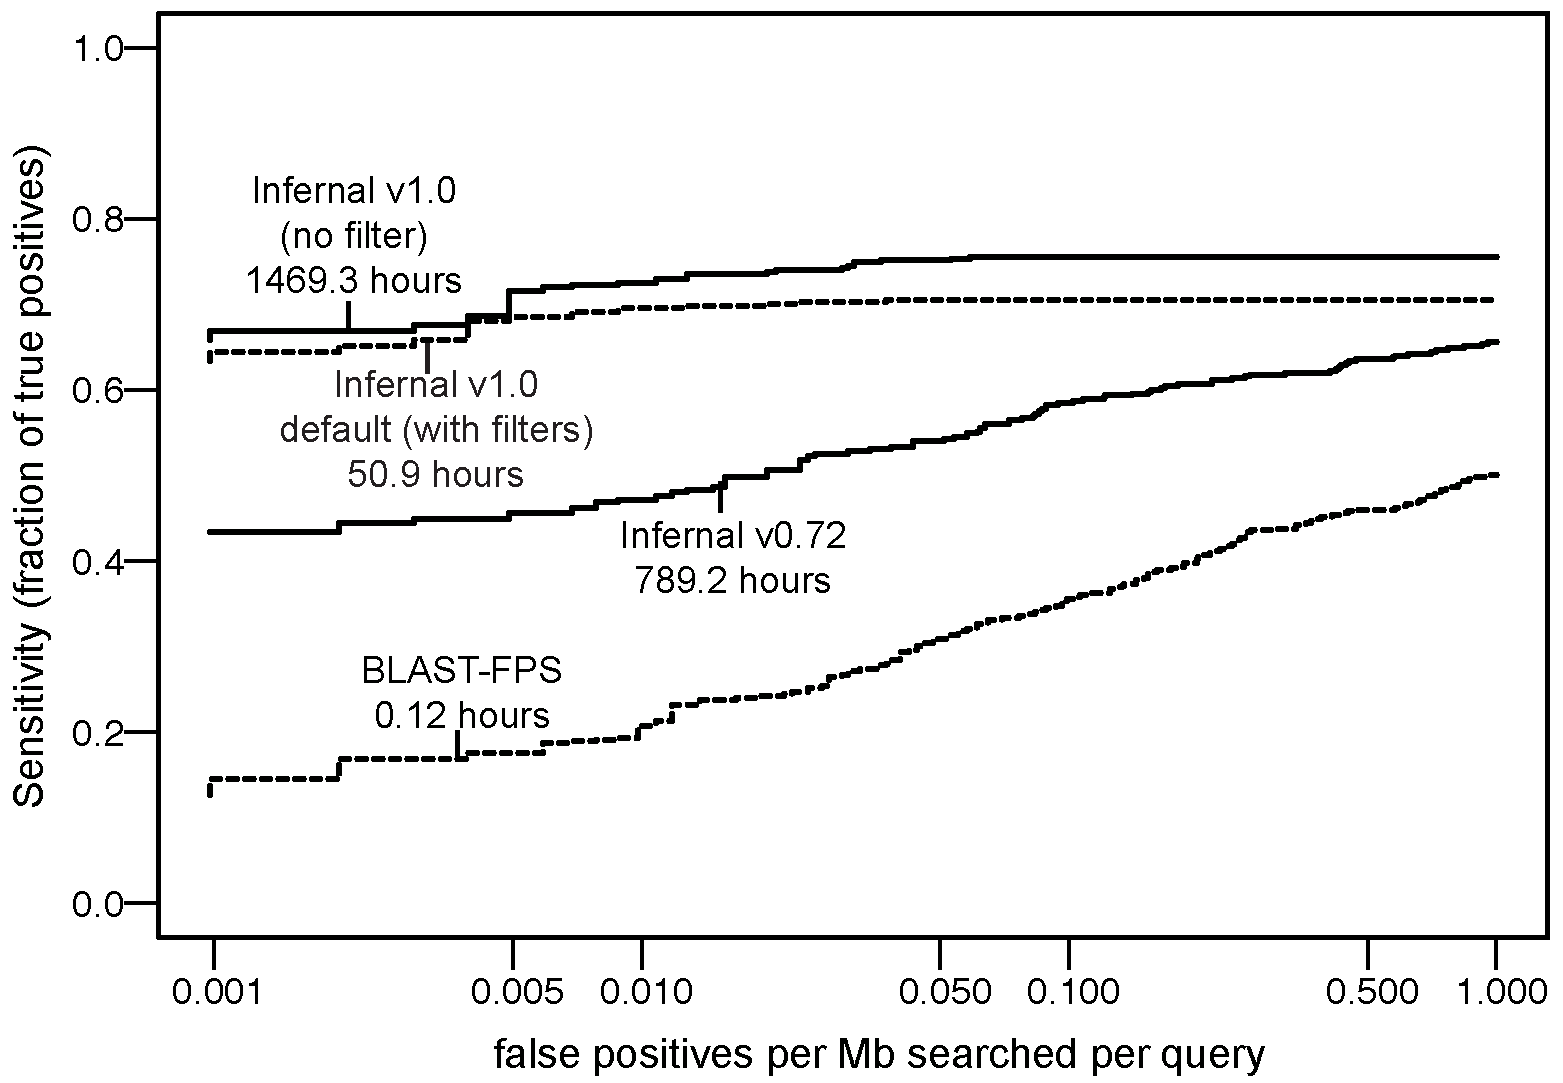
\includegraphics[scale=0.33]{figs/roc}}
\caption{\textbf{ROC curves for the benchmark.}  Plots are shown for
the new \textsc{infernal} 1.0 with and without filters, for the old 
\textsc{infernal} 0.72, and for family-pairwise-searches (FPS) with \textsc{blastn}.}


\label{Fig:01}
\end{figure}

\section*{Acknowledgement}

We thank Goran Ceric for his peerless skill in managing Janelia Farm's
high performance computing resources.

\paragraph{Funding\textcolon} 
\textsc{Infernal} development is supported by Howard Hughes Medical
Institute. It has also been supported in the past by an NIH NHGRI
Institutional Training Grant in Genomic Science (T32-HG000045) to EPN,
an NSF Graduate Fellowship to DLK, and by NIH R01-HG01363 and a
generous endowment from Alvin Goldfarb. 

%%%%%%%%%%%%%%%%%%%%%%%%%%%%%%%%%%%%%%%%%%%%%%%%%%%%%%%%%%%%%%%%%%%%%%%%%%%%%%%%%%%%%
%
%     please remove the " % " symbol from \centerline{\includegraphics{fig01.eps}}
%     as it may ignore the figures.
%
%%%%%%%%%%%%%%%%%%%%%%%%%%%%%%%%%%%%%%%%%%%%%%%%%%%%%%%%%%%%%%%%%%%%%%%%%%%%%%%%%%%%%%

%\bibliographystyle{bioinformatics}
\bibliography{master,books,lab,new}

\end{application}
\end{document}
